%#! platex main.tex

%======================================================================
\chapter{食事行動改善のためのフィードバックシステム}
\label{cha:intervention}

先ほどの章まででは, 食事中の音から食品認識や咀嚼検出を行う手法を提案してきた. 本章では, これらのセンシング手法を用いて食事行動を分析し, 健康的な食事を促進するためのフィードバックシステムについて提案する. 健康的な食事を促進するシステムとして代表的なものは, カロミルやあすけんといった食事管理アプリケーションである. 食事の写真から食品認識を行い, カロリやタンパク質などの栄養素を自動で計算することができ, 日々の食事のバランスを見直すきっかけになる. さらにカロミルでは, 食事・運動・アプリの起動状況などから3ヶ月後の体重を予測する機能も搭載されている. これらのアプリケーションは, スマートフォンのカメラで食事の写真を撮影するだけで利用することができるといった手軽さから広く普及している. しかし, 冒頭でも述べた通り, 食事の内容だけでなく, 食べる順番や速度などの食事行動に関しても, 健康的な食生活を送る上で非常に大切ではある. しかしながら, 既存の食事管理アプリケーションでは, あくまで食事の内容に対する評価しか行うことができない. シャープが開発したbitescanでは, 独自の耳掛け式のウェアラブルデバイスを用いて, 食事中にリアルタイムで咀嚼回数と一口あたりの回数をアプリケーションの画面を通じて確認することができる. さらに, 咀嚼回数やテンポなどが数値化されることで, 自身の食事行動を振り返ることができる. しかし, 独自のウェアラブルデバイスが必要となるため, 普及性に課題があり, そもそも咀嚼回数のみを計測しているため, 食べる順番に対する評価を行うことができない. また, 食べる順番や速度などをアドバイスするために, ウェアラブルデバイスで食事行動を撮影した一人称映像から食事内容をリアルタイムで検出する研究も存在する. しかし, この手法も食事中にカメラで撮影し続ける必要があるため, 一般的な食事シーンで計測を行うのは受け入れ難い. 我々の研究グループでは, 健康的な食生活を促進する行動変容システムとしてeat2picを提案している.\cite{10.1145/3580784} 本研究では, イヤラブルデバイスから食事行動をセンシングし, フィードバックを行うシステムの一例として, eat2picのナッジメカニズムをベースにした咀嚼音から絵を描く「Chew-Draw」インタラクションを提案する.

\begin{figure}[t]
    \begin{center}
        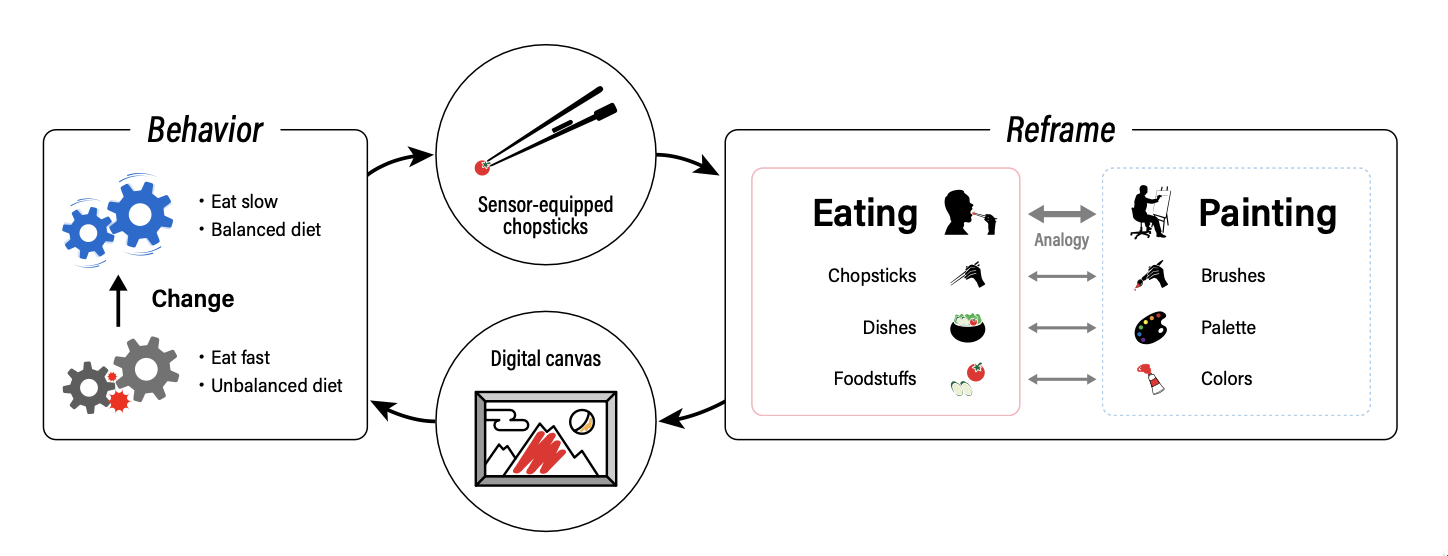
\includegraphics[clip, width=1.0\hsize]{img/eat2pic-concept.png}
        \caption{eat2picのコンセプト}
        \label{fig:eat2pic-concept}
    \end{center}
\end{figure}

\begin{figure}[t]
    \begin{center}
        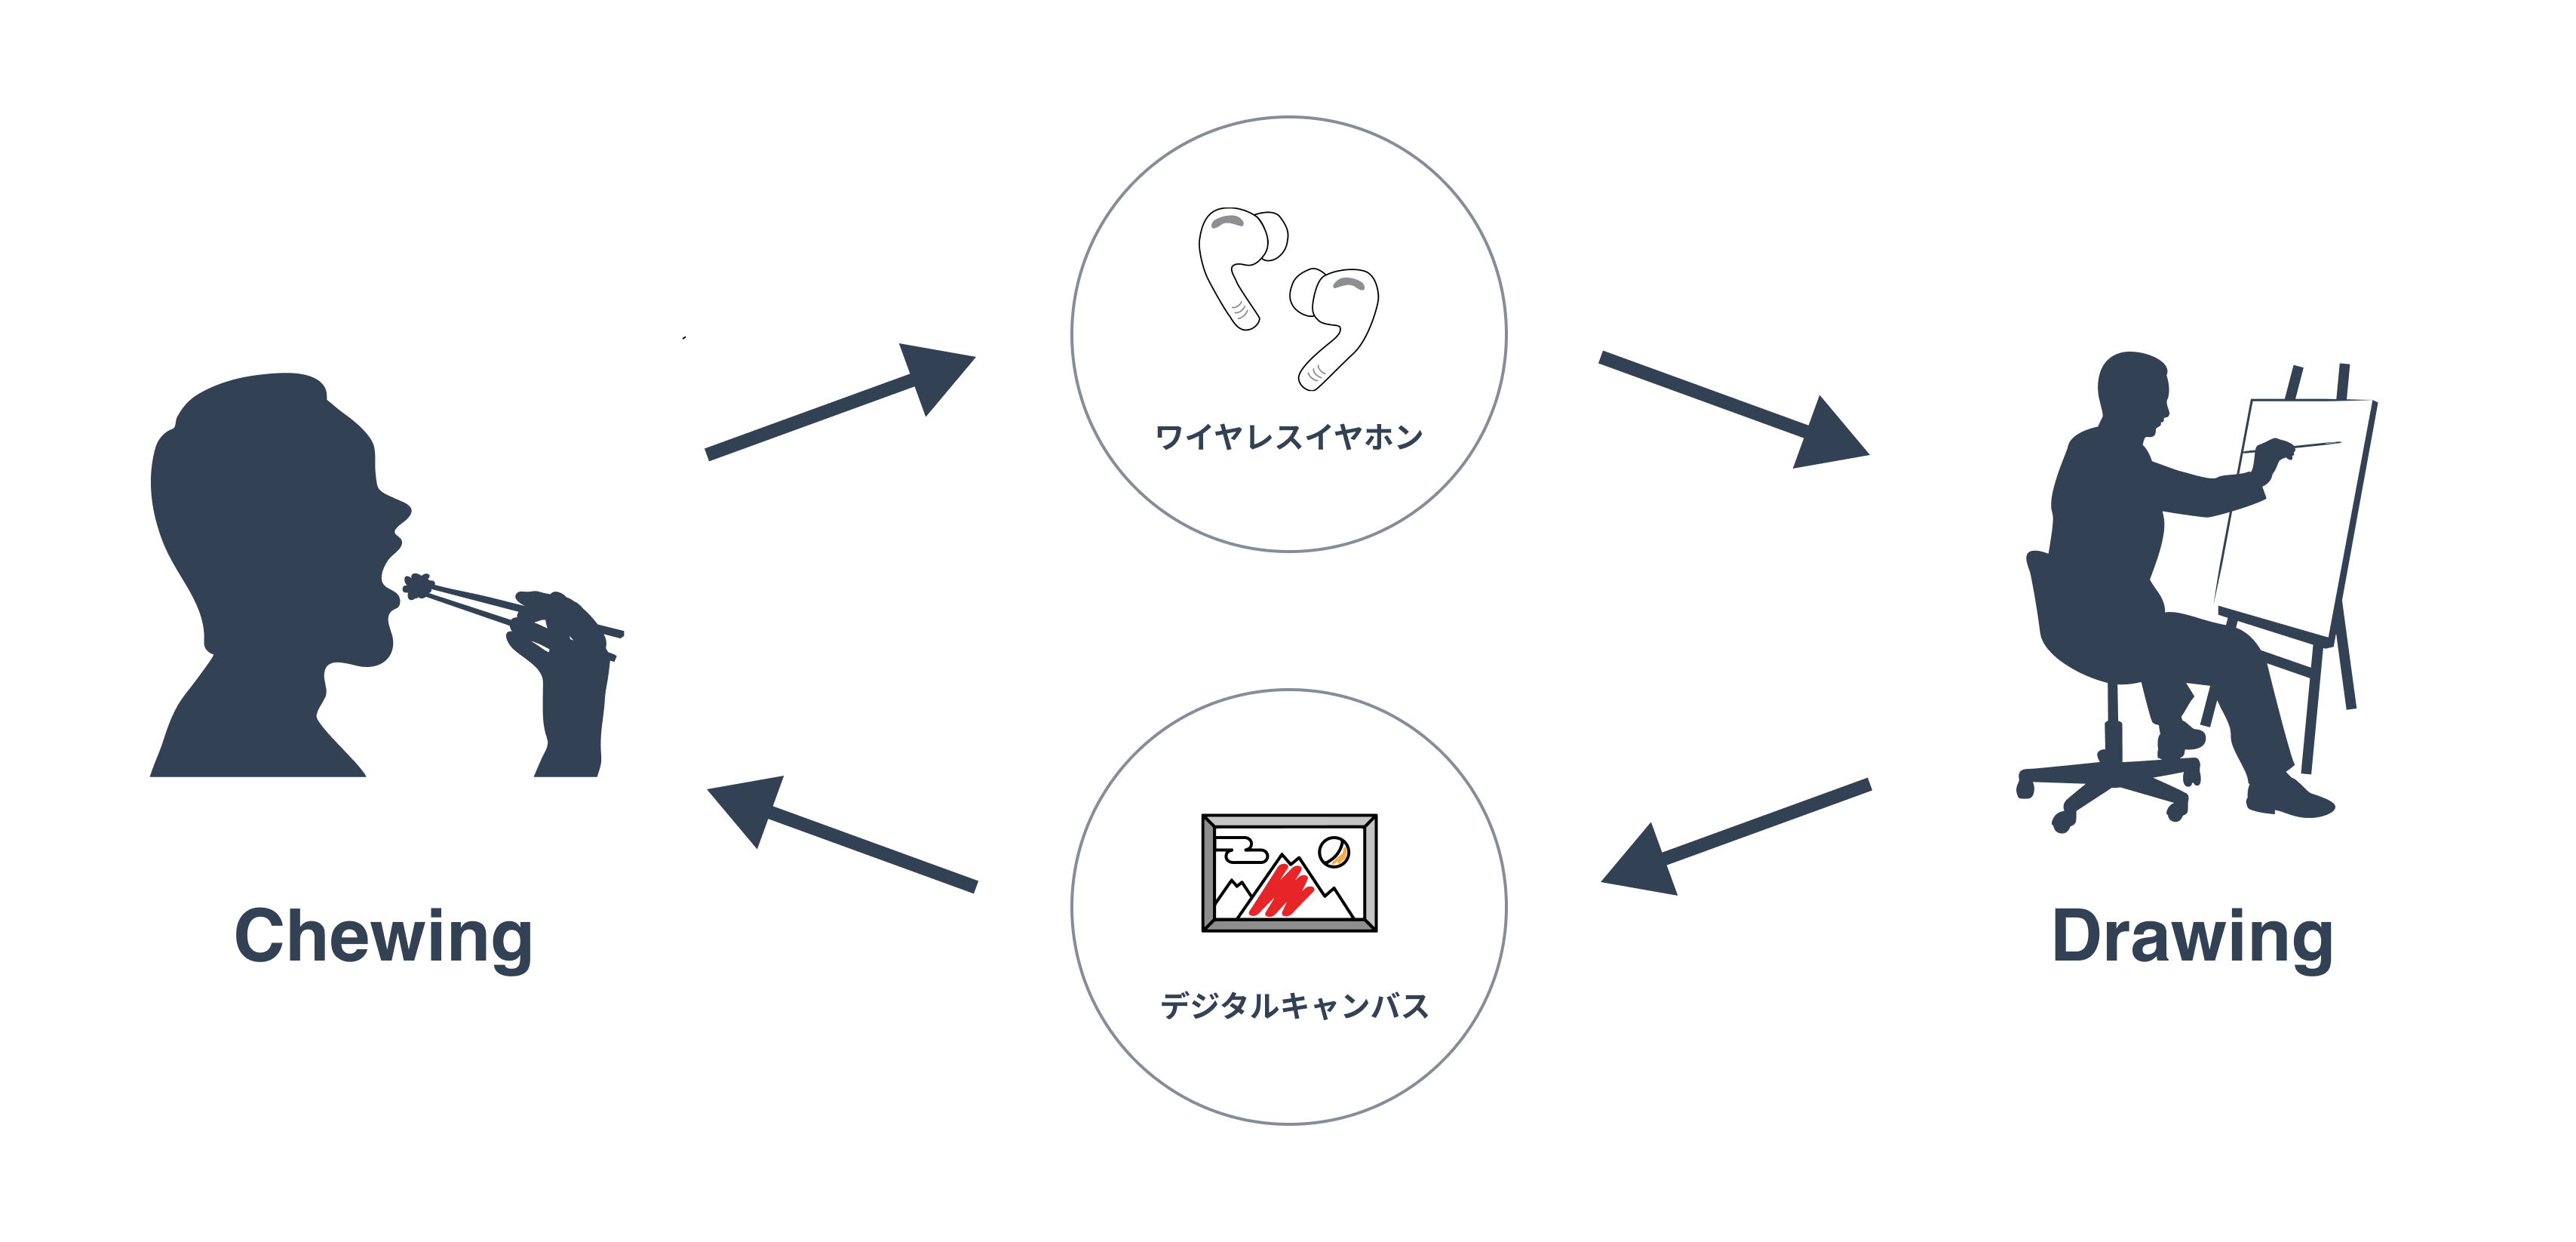
\includegraphics[clip, width=1.0\hsize]{img/chew-draw.png}
        \caption{Chew-Drawインタラクション}
        \label{fig:chew-draw}
    \end{center}
\end{figure}

\section{Chew-Drawインタラクション}

物理世界における「食べる」行動をモニタリングし, それをデジタルな「描く」世界に反映させるナッジングシステム, つまり「食べる」から「描く」をデザインしたeat2picの設計を踏襲する. 図\ref{fig:eat2pic-concept}は, eat2picのコンセプトデザインの概要である. eat2picでは, ほとんどの人が健康的な食習慣を身につけていないのは, 個人的な動機付けの不足, および個人的な成果空間の中での促しが不十分であると仮説を立て, 食べるタスクを他の遊びのタスクに置き換えることでユーザのモチベーションに影響を与え, 健康的な食事行動を促すアプローチを採用している. 具体的にはジャスト・イン・タイム・プロンプトとアンビエント・フィードバックと呼ばれる2種類のナッジメカニズムを採用している. 従来のeat2picではカメラとIMUを搭載した専用の箸型センサを用いて一口ずつ何をどのくらいの速度で食べていたかを自動で追跡し, 食事行動の良し悪しを絵画に表現することで, リアルタイムで視覚的なフィードバックを提供している. 本稿では, eat2picのナッジメカニズムをベースに, 「噛む」動作に応じてデジタルな「描く」世界に反映させる「Chew-Draw」という新たなインタラクションを提案する.(図\ref{fig:chew-draw}) 従来の方法では, 食材を噛むという動作に応じて絵を描くというインタラクションは未対応であったが, eat2picが噛む動作に対応することができれば, 絵を用いた介入によって, よく噛んで食べることといった健康的な食事行動を誘引できる可能性が広がる.

\begin{figure}[t]
    \begin{center}
        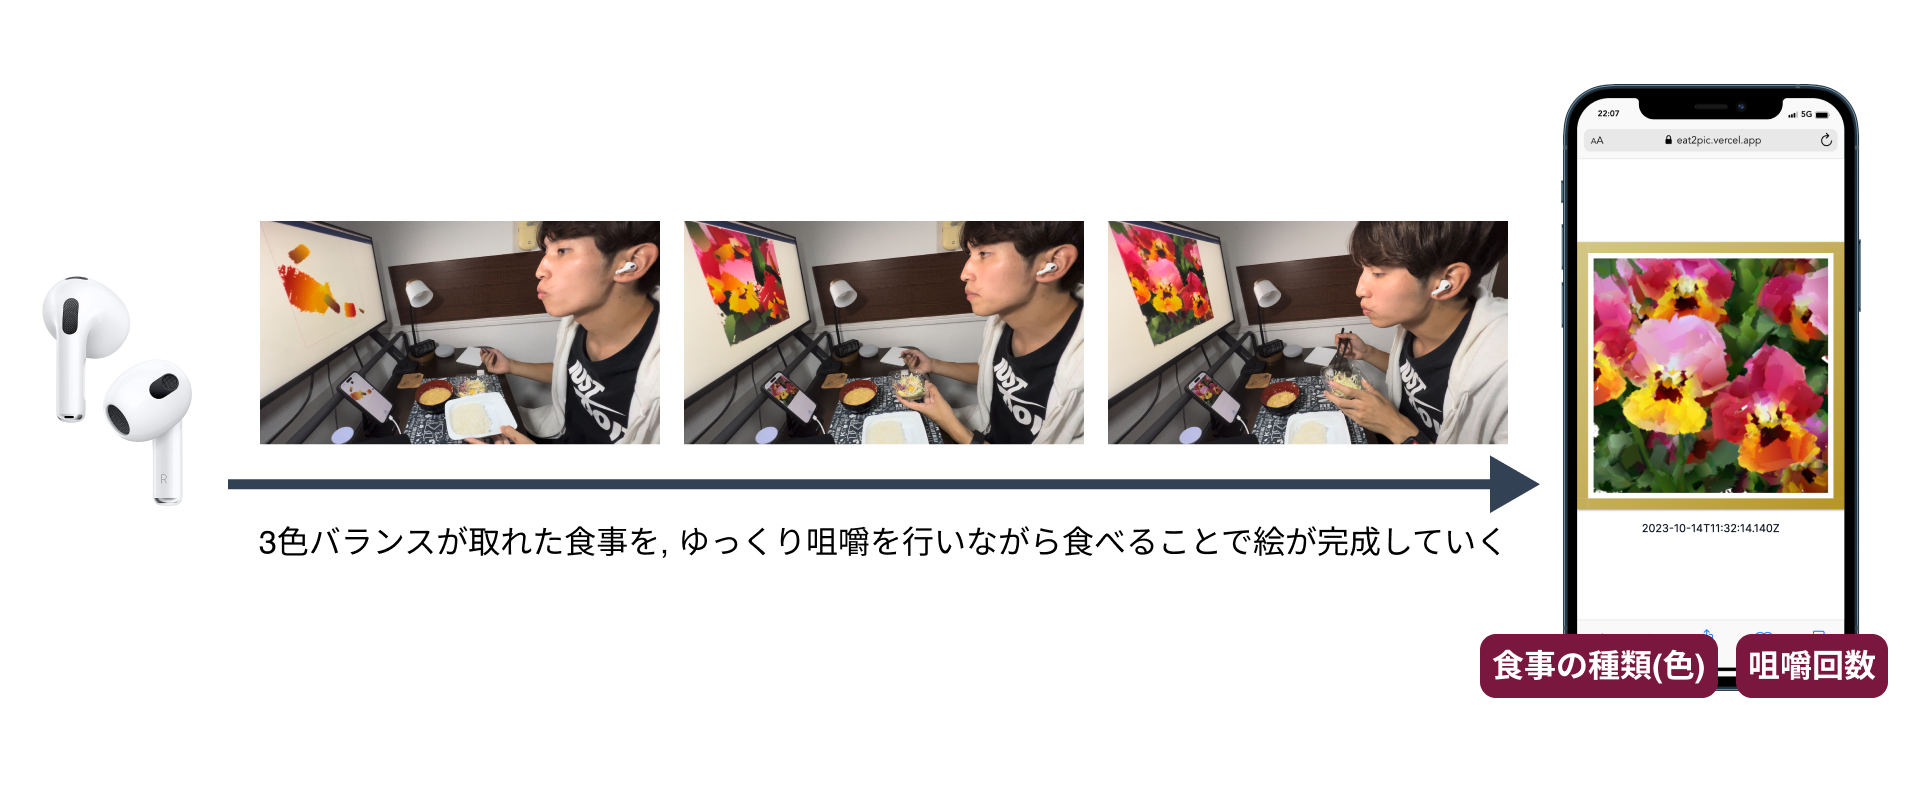
\includegraphics[clip, width=1.0\hsize]{img/chew-draw-eat2pic-system.png}
        \caption{Chew-Drawインタラクションを適用した新たなeat2pic}
        \label{fig:chew-draw-eat2pic-system}
    \end{center}
\end{figure}

\section{システム設計}

図\ref{fig:chew-draw-eat2pic-system}に, Chew-Drawインタラクションを適用した新たなeat2picのシステム概要を示す. 入力デバイスとして独自の箸型センサの代わりに市販のワイヤレスイヤホンを用いる. ワイヤレスイヤホンで得られた食事中の音から食品認識と咀嚼検出を行い, グラフのような定量的な可視化ではなく, ユーザの食べ方に応じて徐々に風景画を着色していくことで健康的な食生活の経過を表現する. また従来のeat2picでは, リアルな額縁の絵画を模したデジタルキャンバスを用いているが, 本稿では, ワイヤレスイヤホンとスマートフォンで完結する利点を活かし, スマートフォン上に同様のデジタルイラストを表示することで, ユーザに視覚的なフィードバックを提供する.

\begin{figure}[t]
    \begin{center}
        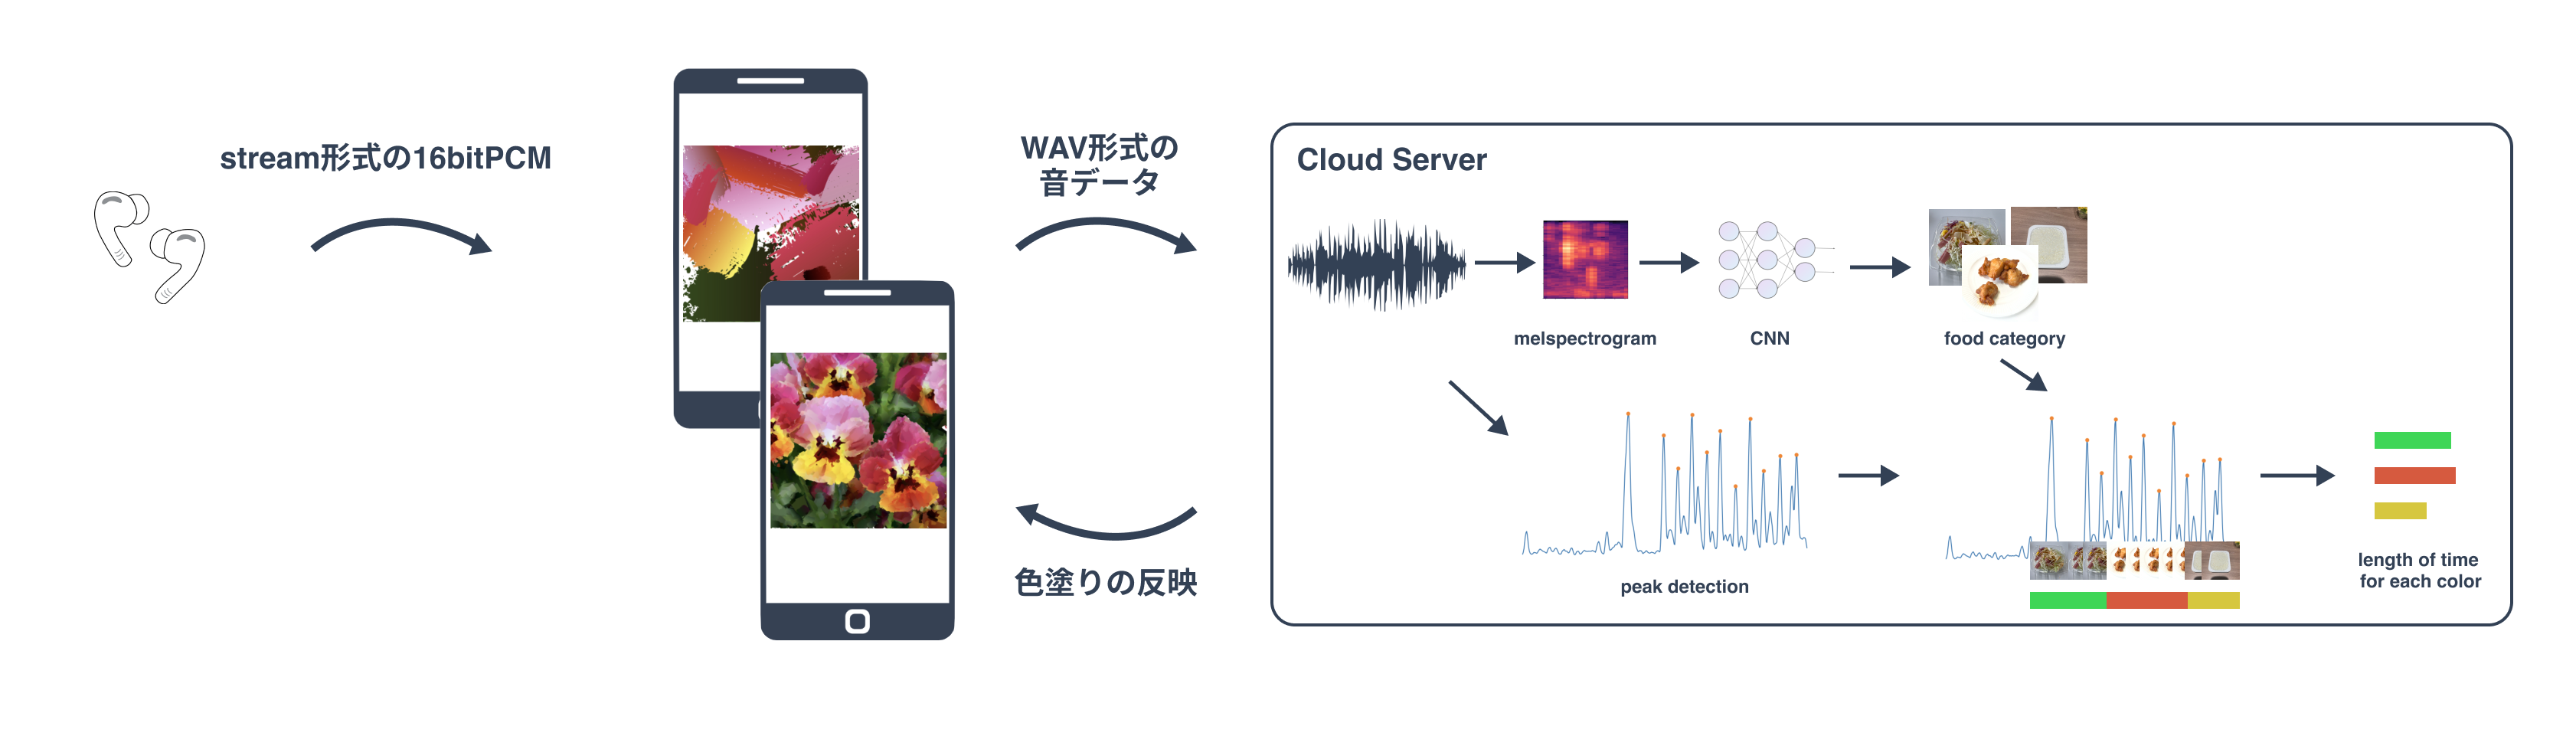
\includegraphics[clip, width=1.0\hsize]{img/eat2pic-impl.png}
        \caption{システム実装}
        \label{fig:eat2pic-impl}
    \end{center}
\end{figure}

\section{アプリケーションの実装}

提案システムは, 市販のワイヤレスイヤホンおよびスマートフォンのみで構成されており, 誰でも利用できるアプリケーションとしてユーザに提供する. 本システムの実装は大きく分けて以下の3つで構成される. システム実装の概要を図\ref{fig:eat2pic-impl}に示す.

\begin{itemize}
    \item 食事中の音をstream形式で録音し, 5秒に1回wav形式のファイルに変換してクラウドサーバに送信
    \item wav形式のファイルから, クラウド上で食品認識と咀嚼検出を行う
    \item 食品認識と咀嚼検出の結果からデジタルキャンバス上に反映
\end{itemize}

ユーザが計測を開始したときに食事中の音をstream形式で収集し続け, 5秒に1回のタイミングでwav形式のファイルに変換し, クラウドサーバに送信する. クラウド上で約5秒間のwav形式の音情報を0.5秒ずつセグメントし食品認識を行い, さらに5秒間の咀嚼タイミングを推定する. 図\ref{fig:app-art}にデジタルキャンバス上に表示される絵の例であるが, この絵は赤・緑・黄の3色で構成されている. 表示される絵はパズルのようにピースで分かれており, 認識した食品を三色食品群に基づき赤・緑・黄にマッピングし, 食品認識と咀嚼検出の結果から, 咀嚼検出のタイミングで対応した食事の色がピースに反映される. つまり, 早食いの場合は色塗りがあまり反映されず, 偏った食事の場合は全体的に単色な絵が完成する. 正しいスピードでバランスの良い食事を行うことで, アプリケーション上の絵が完成するという仕組みとなっている.

%%%%%%%%%%%%%%%%%%%%%%%%%%%%%%%%%%%%%%%%%%%%%%%%
\begin{figure}[t]
    \centering
    \begin{minipage}[b]{0.32\hsize}
        \centering
        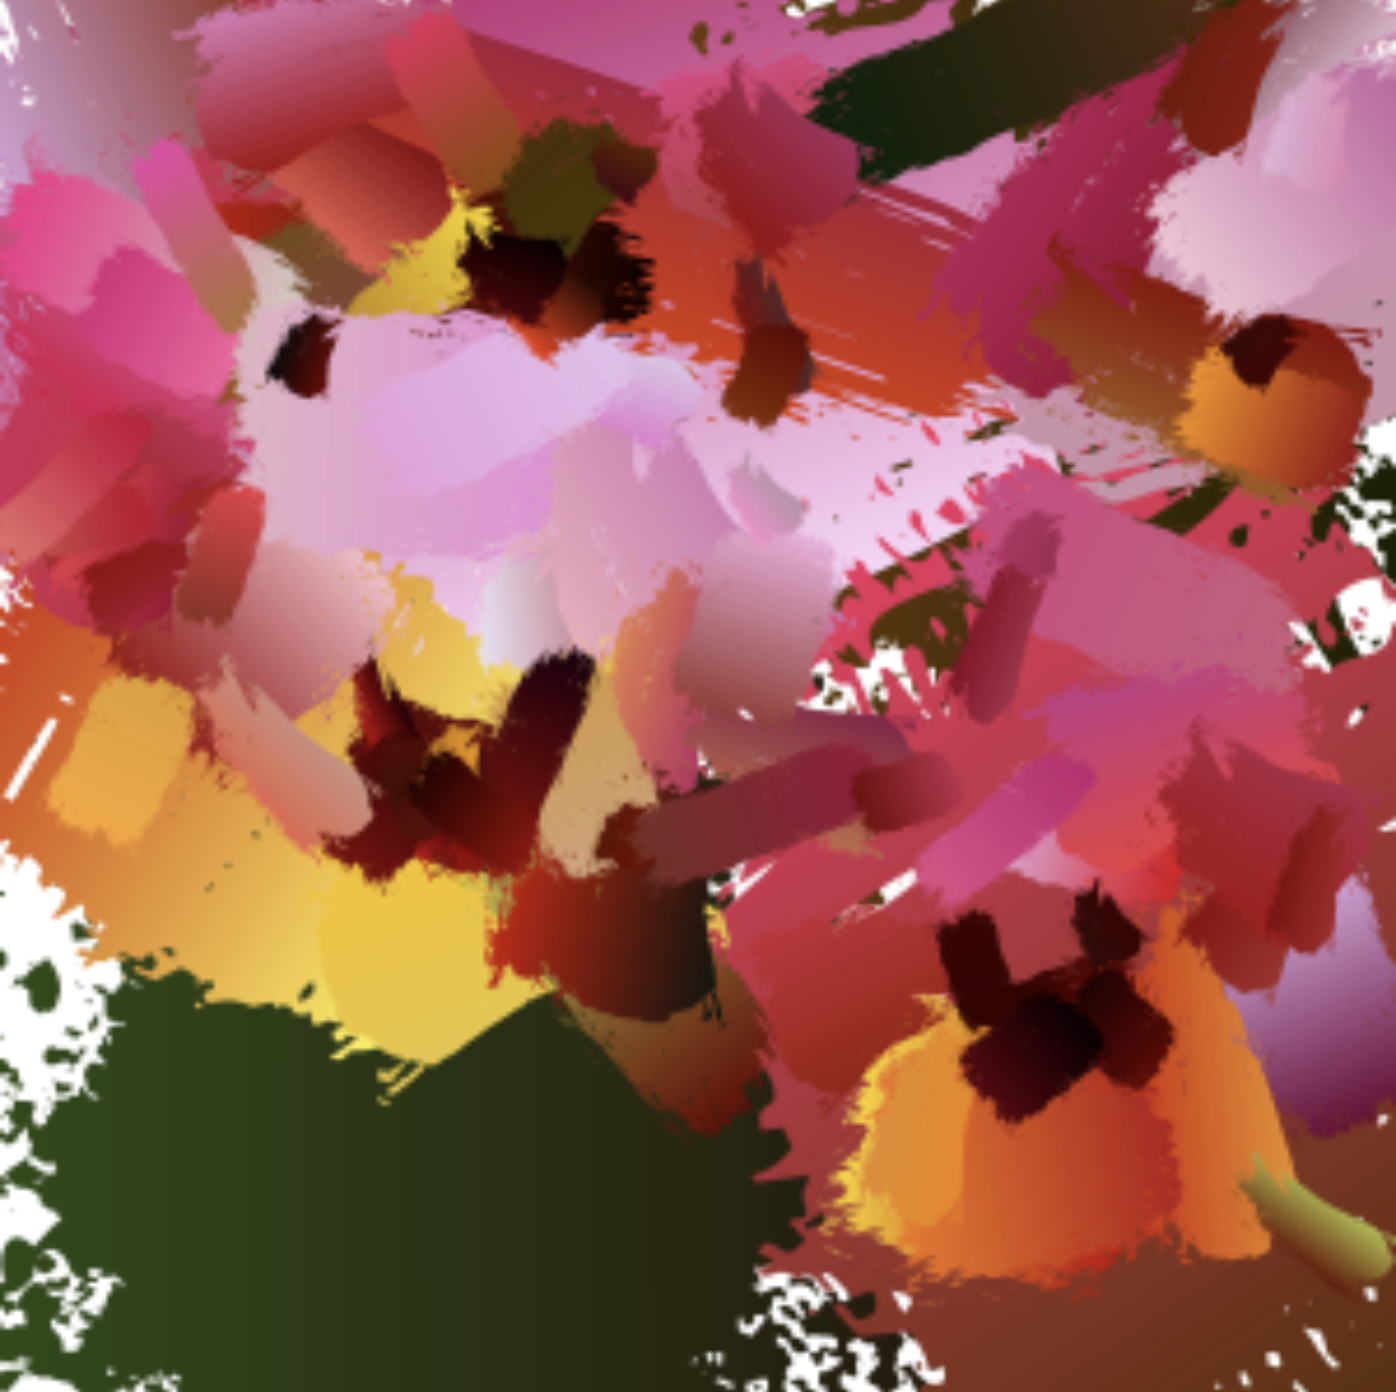
\includegraphics[width=1.0\hsize]{img/art/fast.png}
        \subcaption{早食い}
    \end{minipage}
    \begin{minipage}[b]{0.32\hsize}
        \centering
        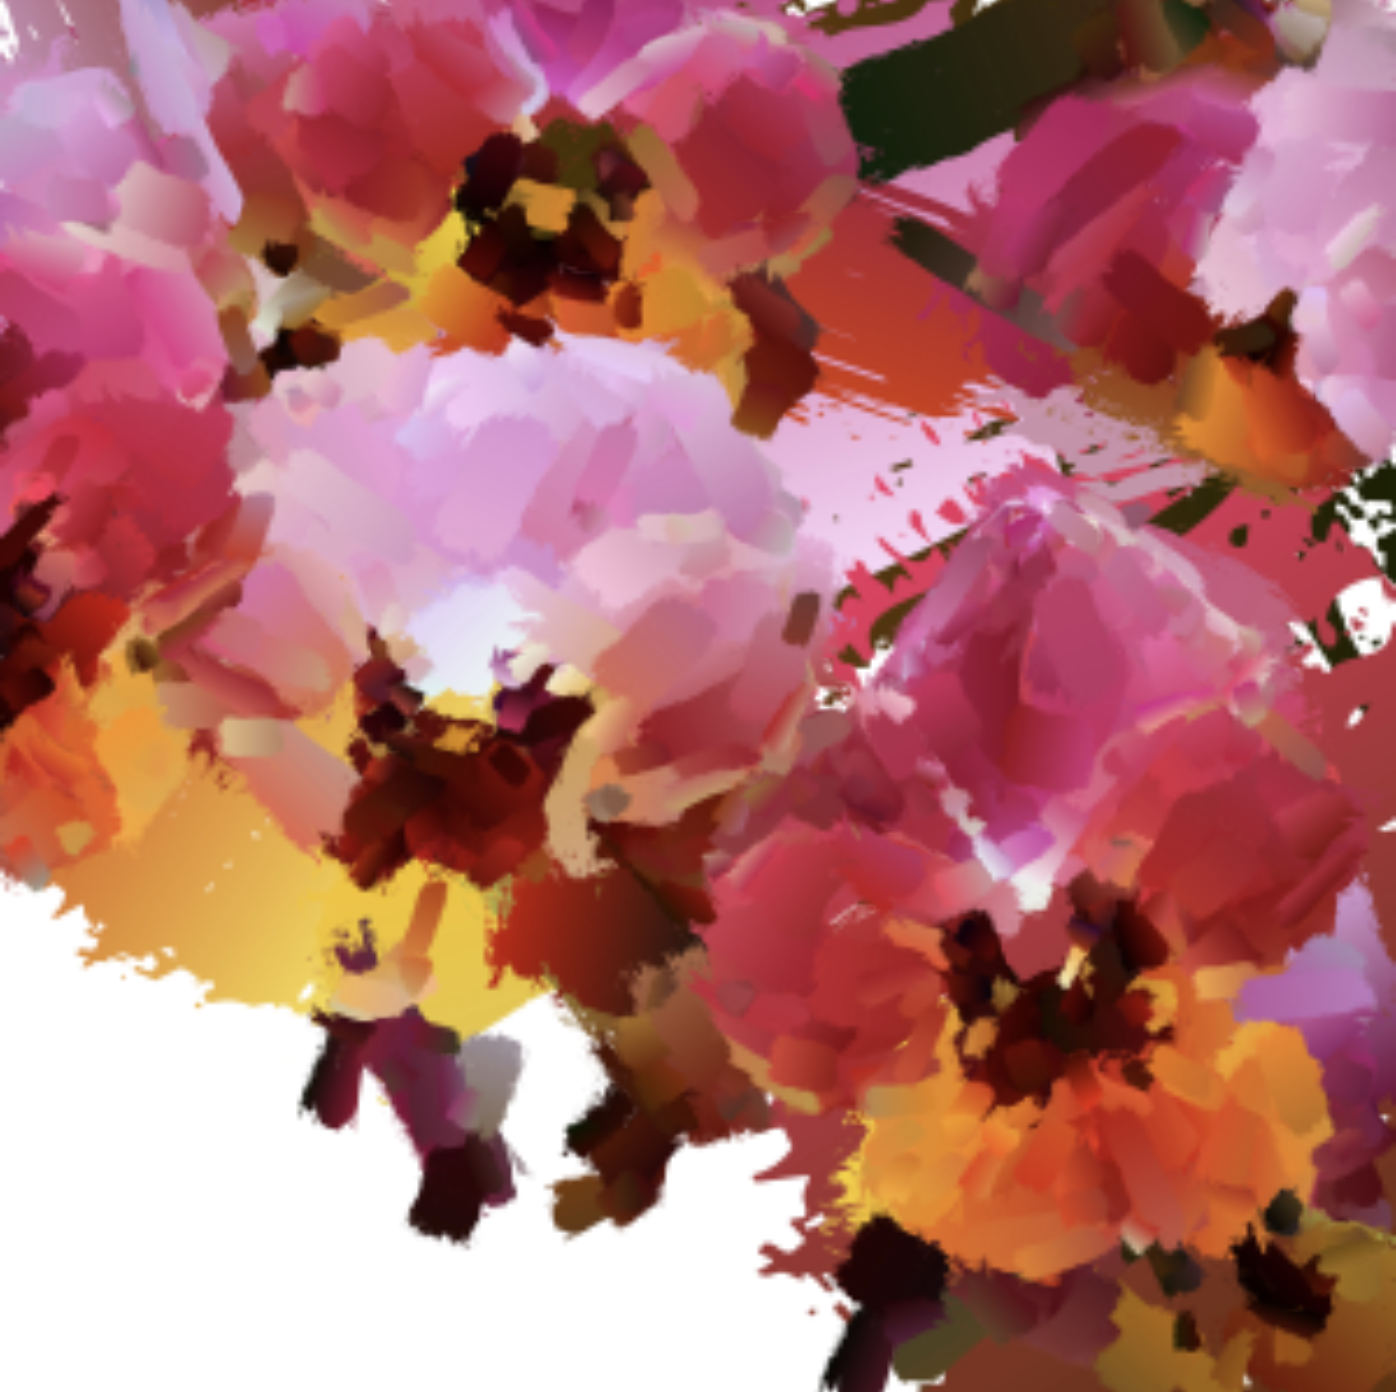
\includegraphics[width=1.0\hsize]{img/art/no-balance.png}
        \subcaption{偏った食事}
    \end{minipage}
    \begin{minipage}[b]{0.32\hsize}
        \centering
        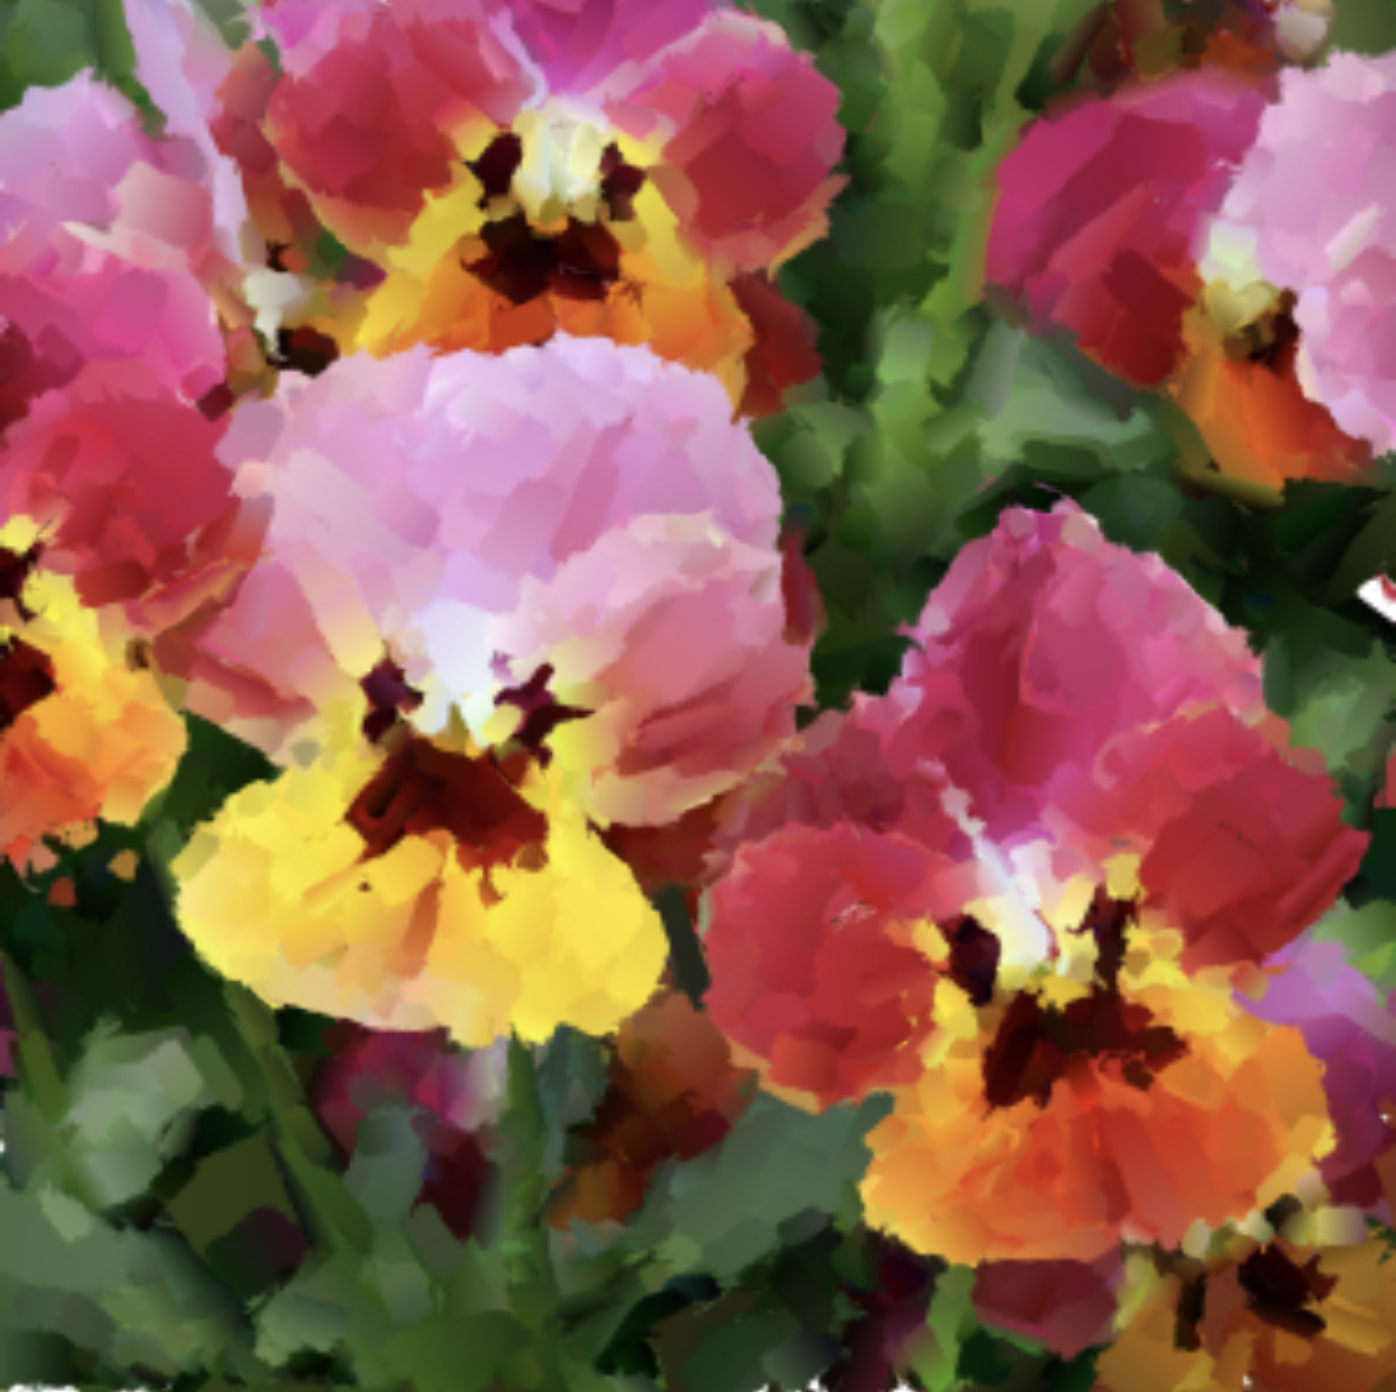
\includegraphics[width=1.0\hsize]{img/art/perfect.png}
        \subcaption{理想的な食事}
    \end{minipage}
    \caption{デジタルキャンバス上に表示される絵の例}
    \label{fig:app-art}
\end{figure}
%%%%%%%%%%%%%%%%%%%%%%%%%%%%%%%%%%%%%%%%%%%%%%%%

\section{アプリケーションの評価}

%%% Local Variables:
%%% mode: yatex
%%% TeX-master: "main"
%%% End:
